\level{2}{ABasicCommunicationTest}

\level{3}{Structure}
{
\centering{}
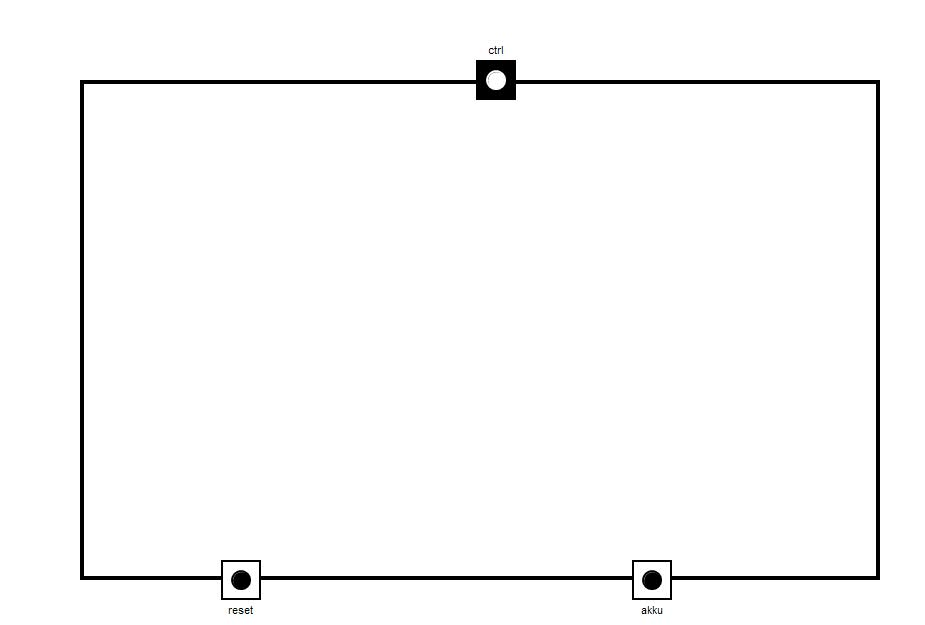
\includegraphics[width=1.0\textwidth]{./images/ABasicCommunicationTest_structure.jpg}
\figcaption{ABasicCommunicationTest Structure}
}

\level{3}{Ports}
\begin{tabular}[ht]{|l|l|l|l|l|p{5cm}|}
\hline
\textbf{Name} & \textbf{Protocol} & \textbf{Type} & \textbf{Kind} & \textbf{Multiplicity} & \textbf{Description}\\
\hline
ctrl & PTestCtrl & reg. & external & 1 & \\
\hline
reset & POnOffTristate & conj. & external & 1 & \\
\hline
akku & PAkkuCtrl & conj. & external & 1 & \\
\hline
\end{tabular}

\level{3}{Behavior}
\level{4}{Top Level}
{
\centering{}
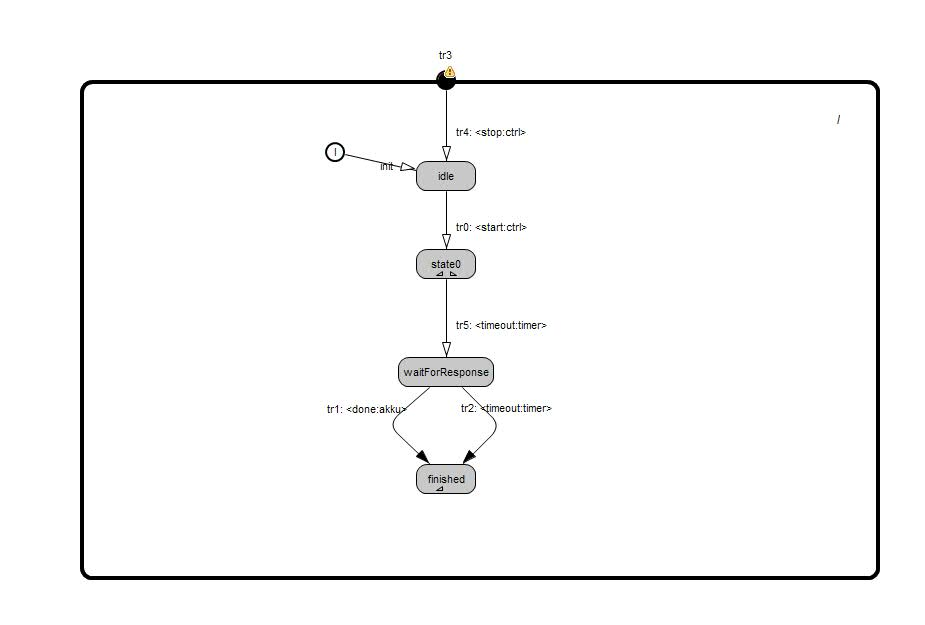
\includegraphics[width=1.0\textwidth]{./images/ABasicCommunicationTest_behavior.jpg}
\figcaption{ABasicCommunicationTest Top State}
}

\begin{par}

\end{par}


\level{3}{Attributes}
\begin{tabular}[ht]{|l|l|p{8cm}|}
\hline
\textbf{Name} & \textbf{Type} & \textbf{Description}\\
\hline
syncTimeout & uint32 & % begin text from user Documentation
Beschreibung
% end text from user Documentation
\\
\hline
errors & uint32 & \\
\hline
testCaseId & uint32 & \\
\hline
\end{tabular}

